\section{Лабараторная работа №2}

\subsection{Структура праекта}

На малюнку \ref{img: lab2} прадстаўлена файлавая структура праекта.

\begin{figure}[h!]
    \centering
    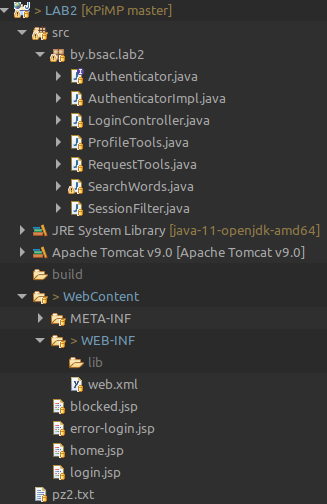
\includegraphics[width=0.5\textwidth]{lab2_structure}
    \caption{Файлавая структура практычнага занятку}
    \label{img: lab2} 
\end{figure}

\subsection{Заданне}

Неабходна рэалізаваць механізм блакіроўкі карыстальніка, які
няверна ўвёў пароль 3 разы, а таксама выводзіць дату і час блакіроўкі.

Дадзенае заданне выконваецца на базе практычнага занятку №2.

\subsubsection{Старонка блакіроўкі blocked.jsp.}

У лістынгу \ref{lst: lab2_blocked} прадстаўлена старонка блакіроўкі
\textit{blocked.jsp}.

\lstinputlisting[caption={Старонка блакіроўкі blocked.jsp},%
                 label={lst: lab2_blocked},%
                 language=HTML5,%
                 style=htmlcssjs]{LAB2/JSP/blocked.jsp}

\subsubsection{Клас RequestTools.}

Дадзены клас забяспечвае механізвы праверкі спроб аўтэнтыфікацыі
ў вэб-праграму і блакіроўкі карыстальніка, калі перавышана колькасць
няверных логінаў ці пароляў.

У лістынгу \ref{lst: lab2_requestTools} прадстаўлены клас
\textit{RequestTools}.

\lstinputlisting[caption={Клас RequestTools},%
                 label={lst: lab2_requestTools},%
                 language=java]{LAB2/Java/RequestTools.java}

\subsubsection{Абноўлены клас фільтра SessionFilter.}

Абноўлены фільтр мае правяраць ці быў заблакаваны карыстальнік,
калі карыстальнік заблакаваны перанакіроўваць на старонку блакіроўкі,
інакш выставіць лічыльнік роўны 0 і перанакіраваць на старонку для
ўвахода.

У лістынгу \ref{lst: lab2_sessionFilter} прадстаўлены абноўлены клас
\textit{SessionFilter}.

\lstinputlisting[caption={Клас SessionFilter},%
                 label={lst: lab2_sessionFilter},%
                 language=java]{LAB2/Java/SessionFilter.java}

\subsubsection{Абноўлены клас LoginController.}

Дабавіў у клас \textit{LoginController} логіку блакіроўкі карыстальніка.

У лістынгу \ref{lst: lab2_loginController} прадстаўлены абноўлены клас
\textit{LoginController}.

\lstinputlisting[caption={Клас LoginController},%
                 label={lst: lab2_loginController},%
                 language=java]{LAB2/Java/LoginController.java}
